
%\section{Introduction}
%\label{sec:introduction}
%
%With the growing adoption of agentic software development environments (e.g., VSCode with GitHub Copilot) and artificial intelligence coding \textit{teammates} \cite{liRiseAITeammates2025}, high-performance computing (HPC) developers are increasingly using large language models (LLMs) to help optimize code. 
%This trend has motivated a growing body of work \cite{liRecentAdvancesDeep, gongLanguageModelsCode2025} on LLM-based code optimization, where LLMs propose source-code and compiler-flag changes to improve performance on a target hardware platform.
%
%\begin{figure}[ht!]
%    \centering
%    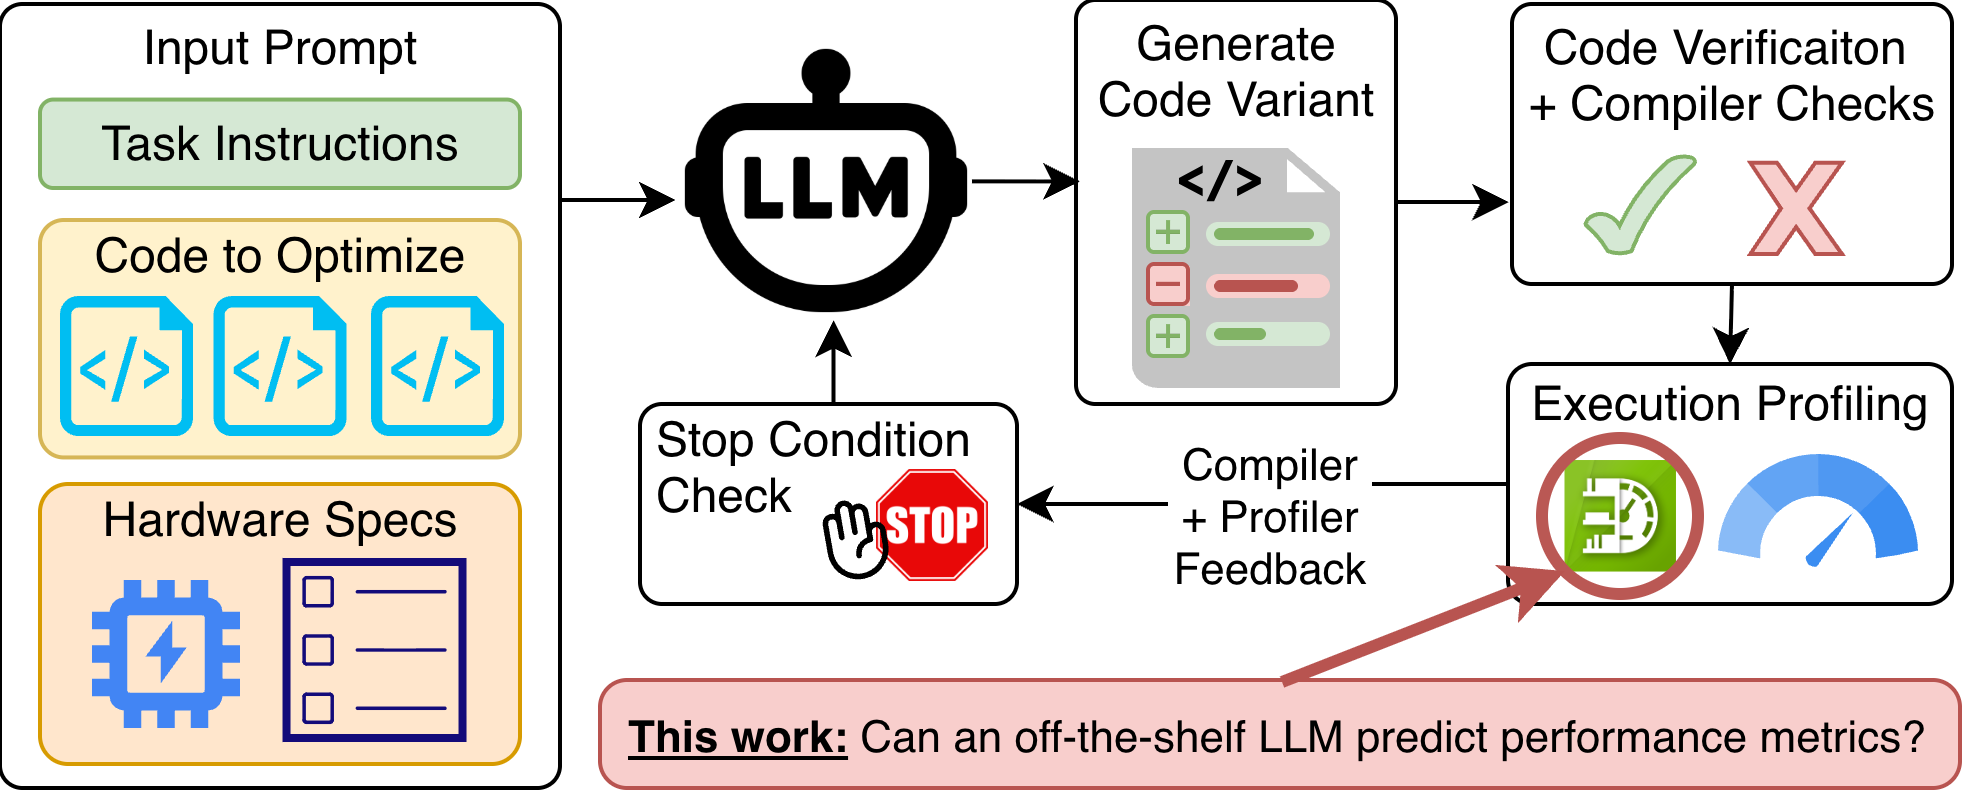
\includegraphics[width=0.95\linewidth]{figures/iterativeCodeOptimizationSimple.drawio.png}
%    \caption{Generalization of typical LLM-based iterative GPU code optimization pipelines where execution feedback from the profiler is used to inform the next code variant generation.
%    This dependence on hardware access for profiler feedback is what we address in this work.}
%    \label{fig:iterativeCodeOptimPipeline}
%\end{figure}
%
%\autoref{fig:iterativeCodeOptimPipeline} visualizes a common feedback-loop design pattern in these systems, where an LLM agent (1) proposes an optimized program variant, (2) profiles the variant on target hardware, (3) incorporates profiler feedback to propose a new variant, and (4) repeats steps 1-3 until a stopping condition is met (e.g., a performance plateau or LLM query budget). 
%Although this iterative profiler-in-the-loop approach has proven to provide better and faster code speedups, it requires repeated hardware access to execute and profile candidate programs.
%
%To reduce this dependence on hardware profiling, an alternative is to estimate performance-relevant signals that can still guide optimization decisions. 
%The Roofline performance model \cite{samuelwilliamsRooflineInsightfulVisual2009} is a standard framework for reasoning about program performance, and \textit{Arithmetic Intensity} (AI) is one of its key metrics. 
%AI captures the balance between computation and data movement, enabling optimizers to reason about whether a program is likely compute-bound or memory-bound. 
%If AI can be estimated directly from program source and artifacts, it may provide useful optimization guidance even when the target hardware is unavailable.
%
%In this paper, we investigate whether state-of-the-art (SoTA) LLMs can address this hardware-accessibility bottleneck for LLM-based GPU kernel optimization pipelines by predicting a Roofline-relevant metric---specifically, arithmetic intensity---across multiple hardware architectures, without direct hardware access. 
%We show that, in many cases, SoTA LLMs can accurately estimate the effective computation-to-communication ratio for 1700 real-world CUDA and OpenMP GPU kernels from the HeCBench suite \cite{HeCBenchMasterZjinlcf}.
%
%
%
%\textbf{Key Question.}
%This work seeks to answer the following question:
%\textit{To what extent can SoTA LLMs act as GPU Roofline performance predictors, from the perspective of predicting a kernel's arithmetic intensity?}
%
%\textbf{Research Questions.} 
%We further break down the key question into four guiding questions:
%\begin{enumerate}
%    \item \textbf{(RQ1) Generalization Across Architectures:} 
%    Can LLMs predict arithmetic intensity well across multiple architectures?
%    \item \textbf{(RQ2) Prompting Strategy:} 
%    Does agentic prompting provide better predictions than zero-shot prompting?
%    \item \textbf{(RQ3) Error Analysis:} 
%    Do certain source code features cause the LLMs to mispredict more than others?
%    \item \textbf{(RQ4) Post-Compilation Artifacts:} 
%    Does including SASS artifacts in LLM inputs improve predictions?
%\end{enumerate}
%
%
%\textbf{Contributions.}
%In summary, this paper makes the following contributions:
%\begin{itemize}
%    \item We show that LLMs can approximate profiler-derived AI for a substantial subset of kernels, enough to support early performance triage.
%    \item We demonstrate the effectiveness of prompting with SASS artifacts to improve the prediction accuracy over prompting with source code alone.
%    \item We find that a plain zero-shot prompting strategy is more cost/time efficient than using an agentic strategy to predict arithmetic intensity.
%    \item We position LLM-based static profiling as a triage tool that complements, rather than replaces, hardware profilers.
%\end{itemize}
%
%The rest of this paper is laid out as follows:
%\autoref{sec:RelatedWorks} gives some insight into the utility of the Roofline performance model for code optimization while also discussing the SoTA LLM-based optimizers that use profiler feedback in their pipelines.
%\autoref{sec:methodology} describes our approach to data collection, prompting, and evaluation metrics.
%\autoref{sec:evaluation} empirically provides answers to our four target research questions.
%Lastly, \autoref{sec:conclusion} provides a discussion of results and future directions for this work.
%
%
%%% additional citations to include in the text
%\cite{wangOmniwisePredictingGPU2025} % omniwise paper
%\cite{boletCanLargeLanguage2025} % bolet LLMs binary categorization Roofline paper
%\cite{nguyen-nhatLLMPerfGPUPerformance2024} % llmperf paper
%\cite{zhangCudaForgeAgentFramework2025} % cudaforge paper
%\cite{leeForecastingGPUPerformance2025} %neusight paper

\newcommand{\rai}[0]{RAI\xspace}

\section{Introduction}
\label{sec:introduction}

% With the growing adoption of agentic software development environments (e.g., VSCode with GitHub Copilot) and artificial intelligence coding \textit{teammates} \cite{liRiseAITeammates2025}, high-performance computing (HPC) developers are increasingly using large language models (LLMs) to help optimize code. 
% This trend has motivated a growing body of work \cite{liRecentAdvancesDeep, gongLanguageModelsCode2025} on LLM-based code optimization, where LLMs propose source-code and compiler-flag changes to improve performance on a target hardware platform.
GPU performance engineering is fundamentally profiler-driven: developers use runtime measurements and hardware counters on target accelerators to determine whether a kernel is limited by computation or data movement, often through Roofline-style analysis \cite{samuelwilliamsRooflineInsightfulVisual2009}. 
In practice, however, this workflow breaks down when the target GPU is unavailable, access is rationed on a shared system, or candidate variants cannot yet be executed end-to-end. 
At the same time, the growing adoption of agentic software development environments and AI coding \textit{teammates} \cite{liRiseAITeammates2025} has motivated a growing body of work on LLM-based code optimization \cite{gongLanguageModelsCode2025}, where LLMs propose source-code and compiler-flag changes to improve performance on a target hardware platform.


% \autoref{fig:iterativeCodeOptimPipeline} visualizes a common feedback-loop design pattern in these systems, where an LLM agent (1) proposes an optimized program variant, (2) profiles the variant on target hardware, (3) incorporates profiler feedback to propose a new variant, and (4) repeats steps 1-3 until a stopping condition is met (e.g., a performance plateau or LLM query budget). 
% Although this iterative profiler-in-the-loop approach has proven to provide better and faster code speedups, it requires repeated hardware access to execute and profile candidate programs.
\autoref{fig:iterativeCodeOptimPipeline} visualizes a common iterative feedback-loop design pattern in these systems, where an LLM agent (1) proposes an optimized program variant, (2) profiles the variant on target hardware, (3) incorporates profiler feedback to propose a new variant, and (4) repeats steps 1--3 until a stopping condition is met (e.g., a performance plateau or LLM query budget). 
Although this iterative profiler-in-the-loop approach can improve code speedups, it also tightly couples optimization quality to repeated hardware access for execution and profiling. 
This dependency is especially problematic for early-stage kernel development, where developers would ideally like useful performance guidance before investing scarce accelerator time.

% To reduce this dependence on hardware profiling, an alternative is to estimate performance-relevant signals that can still guide optimization decisions. 
% The Roofline performance model \cite{samuelwilliamsRooflineInsightfulVisual2009} is a standard framework for reasoning about program performance, and \textit{Arithmetic Intensity} (AI) is one of its key metrics. 
% AI captures the balance between computation and data movement, enabling optimizers to reason about whether a program is likely compute-bound or memory-bound. 
% If AI can be estimated directly from program source and artifacts, it may provide useful optimization guidance even when the target hardware is unavailable.
An alternative to hardware profiling is to estimate a smaller, interpretable performance signal that can still guide optimization decisions. 
%The Roofline performance model \cite{samuelwilliamsRooflineInsightfulVisual2009} is a standard framework for reasoning about program performance, and \textit{arithmetic intensity} (\textbf{AI}) is one of its central quantities. 
The Roofline performance model \cite{samuelwilliamsRooflineInsightfulVisual2009} is a standard framework for reasoning about program performance, and \textit{\textbf{R}oofline \textbf{A}rithmetic \textbf{I}ntensity} (\textbf{\rai}) is one of its central quantities. 
\rai captures the balance between computation and data movement, making it an actionable signal for deciding whether optimization efforts should focus on reducing memory traffic or improving computational efficiency. 
Recent work has begun to explore whether LLMs can reason about Roofline-relevant properties from code, including coarse categorization of kernels as memory-bound or compute-bound \cite{boletCanLargeLanguage2025}. 
Here, we push that idea further by asking whether LLMs can estimate a quantitative Roofline metric directly from program representations, even when target hardware is unavailable.

\begin{figure}[t!]
    \centering
    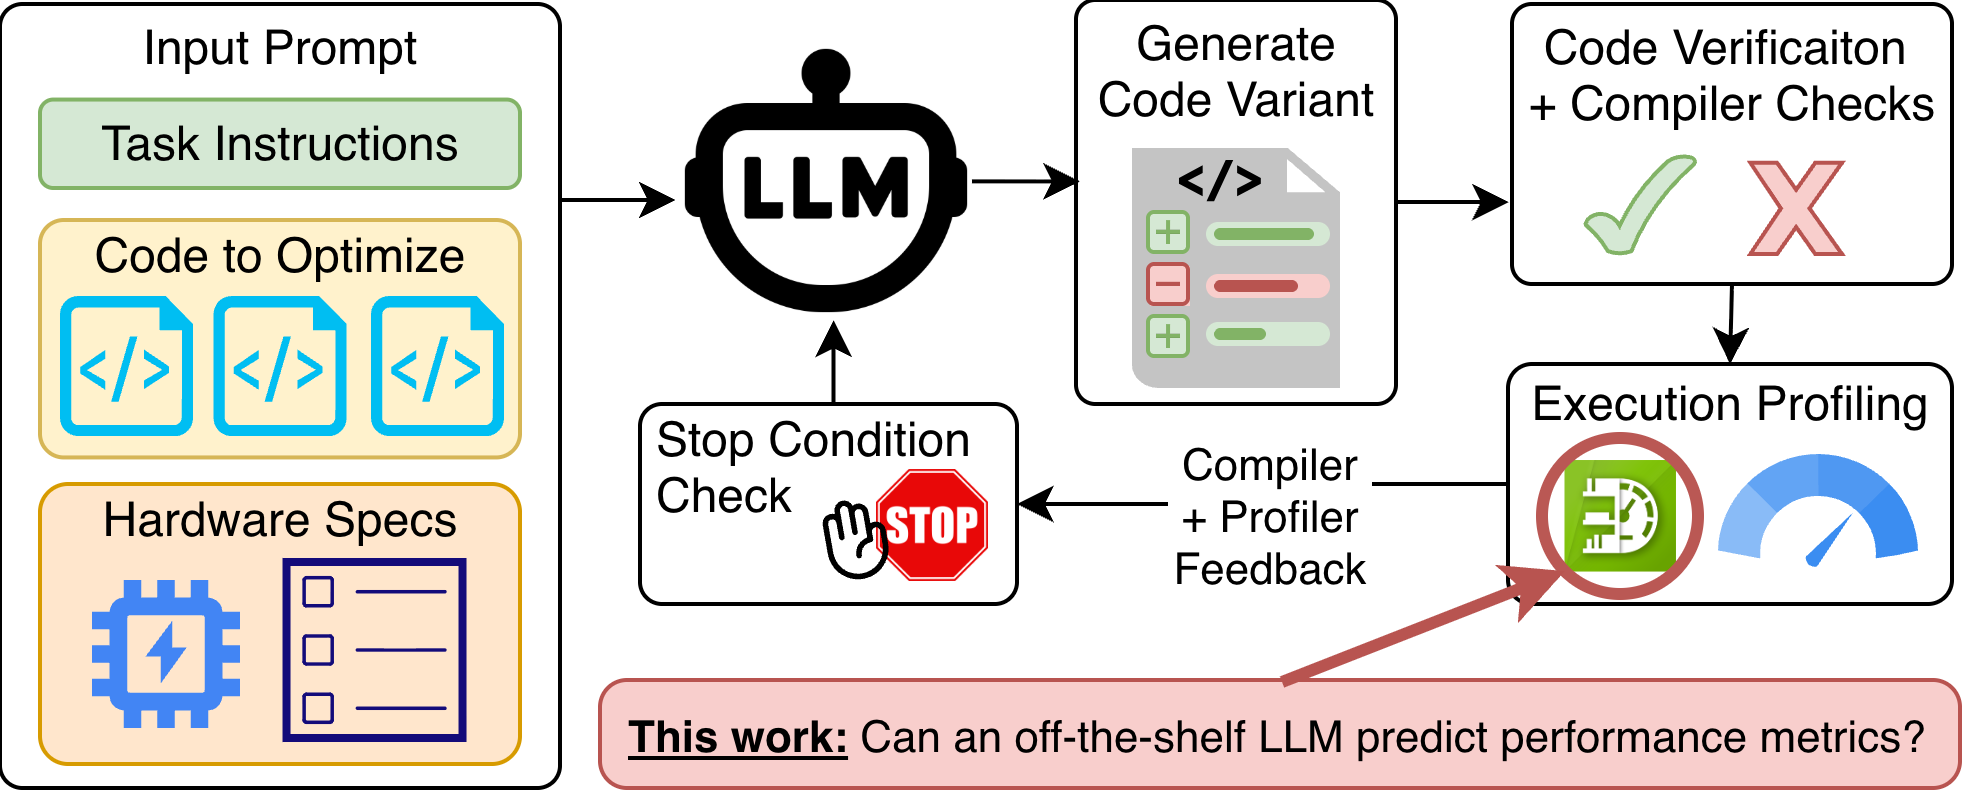
\includegraphics[width=0.95\linewidth]{figures/iterativeCodeOptimizationSimple.drawio.png}
    %\caption{Generalization of typical LLM-based iterative GPU code optimization pipelines where execution feedback from the profiler is used to inform the next code variant generation.
    %This dependence on hardware access for profiler feedback is what we address in this work.}
    \caption{Typical iterative LLM-based GPU optimization loop: generate a code variant, profile it on target hardware, and use the resulting feedback to guide the next variant.
    Our work targets the hardware-access bottleneck in this loop by estimating a Roofline-relevant signal before profiling.}
    \label{fig:iterativeCodeOptimPipeline}
\end{figure}

The main challenge with estimating \rai from source code is that effective \rai is not always obvious from source code alone: compiler passes such as lowering, instruction selection, transcendental expansion, and other low-level transformations can modify compute and memory load in ways that are not explicit from the source code \cite{alfredCompilersPrinciplesTechniques2007}. 
This makes \rai prediction a challenging test of LLMs' ability to recover profiler-relevant behavior from source-level structure alone. 
Nevertheless, we also study whether post-compilation artifacts such as SASS (i.e.: GPU assembly instructions) can help LLMs to accurately predict the \rai, as such artifacts would reveal the effects of compiler passes on the source code to the LLMs.

% In this paper, we investigate whether state-of-the-art (SoTA) LLMs can address this hardware-accessibility bottleneck for LLM-based GPU kernel optimization pipelines by predicting a Roofline-relevant metric---specifically, arithmetic intensity---across multiple hardware architectures, without direct hardware access. 
% We show that, in many cases, SoTA LLMs can accurately estimate the effective computation-to-communication ratio for 1700 real-world CUDA and OpenMP GPU kernels from the HeCBench suite \cite{HeCBenchMasterZjinlcf}.
%In this paper, we investigate whether off-the-shelf LLMs can address this hardware-accessibility bottleneck for GPU kernel optimization pipelines by predicting a Roofline-relevant metric---specifically, profiled arithmetic intensity---across multiple GPU architectures, without direct hardware access. 
%Unlike recent work that fine-tunes LLMs for GPU metric prediction~\cite{wangOmniwisePredictingGPU2025} or studies broader GPU performance modeling~\cite{leeForecastingGPUPerformance2025, nguyen-nhatLLMPerfGPUPerformance2024}, our goal is to test the zero-training regime: can LLMs, used as-is through prompting alone, reason about GPU kernel performance and serve as useful Roofline-oriented triage tools. 
In this paper, we investigate whether off-the-shelf LLMs can help address this hardware-accessibility bottleneck by predicting a single Roofline-relevant quantity---profiled arithmetic intensity---well enough to support early GPU-kernel triage without direct hardware access.
Unlike prior work that either predicts only coarse Roofline classes~\cite{boletCanLargeLanguage2025}, fine-tunes models for GPU metric prediction~\cite{wangOmniwisePredictingGPU2025}, or studies broader GPU performance modeling~\cite{leeForecastingGPUPerformance2025, nguyen-nhatLLMPerfGPUPerformance2024}, our focus is deliberately narrow: quantitative \rai prediction in the zero-training regime, using off-the-shelf LLMs through prompting alone.
Specifically, this work seeks to answer the following key question:
\textit{To what extent can off-the-shelf LLMs, used without task-specific training or fine-tuning, act as GPU Roofline triage tools by predicting a kernel's Roofline Arithmetic Intensity?}
We evaluate this question on 254 real-world CUDA and OpenMP GPU kernels from the HeCBench suite~\cite{HeCBenchMasterZjinlcf} across four different NVIDIA GPU architectures: an RTX 3080, A10, A100, and H100.
%Our results reveal that, for a substantial subset of kernels, modern LLMs can approximate effective computation-to-data-movement ratios well enough to match ground-truth profiler metrics.
We highlight three direct findings up front:
\textbf{(1)} Prompts that include post-compilation information substantially improve half-precision \rai estimates and compute/bandwidth-bound classifications for the stronger models.
\textbf{(2)} The strongest overall results come from the more capable (expensive) models, but a much cheaper model remains surprisingly competitive when only pre-compilation information is available.
\textbf{(3)} Prediction quality is not uniform: larger-cache GPUs are easier settings than smaller-cache GPUs, and prediction errors concentrate around code patterns such as division, transcendental math functions, reusable subexpressions, and loop-invariant floating-point work.

%\textbf{Key Question.}
% This work seeks to answer the following question:
% \textit{To what extent can SoTA LLMs act as GPU Roofline performance predictors, from the perspective of predicting a kernel's arithmetic intensity?}
% This work seeks to answer the following question:
% \textit{To what extent can off-the-shelf SoTA LLMs, used without task-specific training or fine-tuning, act as GPU Roofline triage tools by predicting a kernel's arithmetic intensity?}

\textbf{Research Questions.} 
We further break down the above key question into three guiding questions:
\begin{enumerate}
    \item \textbf{(RQ1) Generalization Across Architectures:} 
    Can LLMs predict Roofline Arithmetic Intensity well across multiple architectures?
    \item \textbf{(RQ2) Error Analysis:} 
    Do certain source code features cause the LLMs to mispredict more than others?
    \item \textbf{(RQ3) Post-Compilation Artifacts:} 
    Does feeding SASS artifacts to LLMs improve predictions?
\end{enumerate}


\textbf{Contributions.}
This paper makes the following contributions:
\begin{itemize}
    % \item We show that LLMs can approximate profiler-derived AI for a substantial subset of kernels, enough to support early performance triage.
    % \item We demonstrate the effectiveness of prompting with SASS artifacts to improve the prediction accuracy over prompting with source code alone.
    % \item We find that a plain zero-shot prompting strategy is more cost/time efficient than using an agentic strategy to predict arithmetic intensity.
    % \item We position LLM-based static profiling as a triage tool that complements, rather than replaces, hardware profilers.
    % \item We compare zero-shot prompting against an agentic prompting strategy and show when the additional reasoning cost of agentic interaction is, and is not, worthwhile for arithmetic-intensity prediction.

    \item We show that off-the-shelf LLMs, without task-specific training or fine-tuning, can estimate a kernel's arithmetic intensity well enough to provide useful early Roofline triage across multiple GPU architectures.
    \item We show that adding post-compilation artifacts improves prediction quality, especially for half-precision estimates and for deciding whether a kernel falls on the bandwidth- or compute-limited side of the Roofline, thereby quantifying when source-level reasoning fails to capture compiler-realized behavior.
    \item We identify where the method is (and is not) reliable by comparing inexpensive and premium LLMs across CUDA and OpenMP kernels, across GPUs with different cache regimes, and across source-code features that systematically raise prediction error.
    \item We release a benchmark for quantitative, hardware-free Roofline reasoning that includes GPU kernels, compilation and execution context, post-compilation artifacts, and profiler-derived ground truth for arithmetic-intensity prediction.\footnote{https://flopbench.github.io/}

    % \item We demonstrate that off-the-shelf LLMs can indeed estimate a kernels' arithmetic intensity across multiple GPU architectures, without any task-specific training or fine-tuning.
    % \item We show that including SASS artifacts during prompting can improve prediction accuracy over source code-only prompting, quantifying when source-level reasoning fails to capture compiler-realized behavior.
    % \item We differentiate the source code features of both CUDA and OpenMP codes that contribute to better (or worse) arithmetic intensity predictions. 
    % \item We compare and contrast the effectiveness of inexpensive and premium LLMs for the prediction task, highlighting the trade-off between query cost and prediction accuracy.
    % \item We identify a property of GPU hardware that hinders LLM prediction accuracy
    % \item We publish our dataset of GPU kernels as a benchmark that can be used to gauge LLM proficiency in this prediction task.
    
    % \item We evaluate whether off-the-shelf LLMs can estimate profiler-derived arithmetic intensity across multiple GPU architectures, without any task-specific training or fine-tuning.
    % \item We delineate the code features of both CUDA and OpenMP codes that contribute to better (or worse) prediction results.
    % \item We position LLM-based static profiling as an early performance-triage tool that complements, rather than replaces, hardware profilers.
\end{itemize}

% The rest of this paper is laid out as follows:
% \autoref{sec:RelatedWorks} gives some insight into the utility of the Roofline performance model for code optimization while also discussing the SoTA LLM-based optimizers that use profiler feedback in their pipelines.
% \autoref{sec:methodology} describes our approach to data collection, prompting, and evaluation metrics.
% \autoref{sec:evaluation} empirically provides answers to our four target research questions.
% Lastly, \autoref{sec:conclusion} provides a discussion of results and future directions for this work.
The rest of this paper is organized as follows:
\autoref{sec:RelatedWorks} reviews the utility of the Roofline performance model for code optimization, related static and learned GPU performance predictors, and recent LLM-based optimization systems that depend on profiler feedback.
\autoref{sec:methodology} describes our approach to data collection, prompting, and evaluation metrics.
\autoref{sec:evaluation} empirically answers our research questions.
Lastly, \autoref{sec:conclusion} discusses the implications of our findings and future directions for this work.


